%%%%%%%%%%%%%%%%%%%%%%%%%%%%%%%%%%%%%%%%%
% University/School Laboratory Report
% LaTeX Template
% Version 3.1 (25/3/14)
%
% This template has been downloaded from:
% http://www.LaTeXTemplates.com
%
% Original author:
% Linux and Unix Users Group at Virginia Tech Wiki 
% (https://vtluug.org/wiki/Example_LaTeX_chem_lab_report)
%
% License:
% CC BY-NC-SA 3.0 (http://creativecommons.org/licenses/by-nc-sa/3.0/)
%
%%%%%%%%%%%%%%%%%%%%%%%%%%%%%%%%%%%%%%%%%

%----------------------------------------------------------------------------------------
%	PACKAGES AND DOCUMENT CONFIGURATIONS
%----------------------------------------------------------------------------------------

\documentclass{article}

\usepackage[version=3]{mhchem} % Package for chemical equation typesetting
\usepackage{siunitx} % Provides the \SI{}{} and \si{} command for typesetting SI units
\usepackage{graphicx} % Required for the inclusion of images
\usepackage{natbib} % Required to change bibliography style to APA
\usepackage{amsmath} % Required for some math elements 
\usepackage{enumerate} % Required for the enumerate function
\usepackage[siunitx]{circuitikz} % Required for the drawing of circuit diagrams
\usepackage{caption}
\usepackage{graphicx}
\usepackage{subcaption}
\usepackage{xfrac}
\usepackage{float}
\usepackage{enumitem}
\usepackage{chemgreek}
\usepackage{pgfplots}

\setlength\parindent{0pt} % Removes all indentation from paragraphs

\renewcommand{\labelenumi}{\alph{enumi}.} % Make numbering in the enumerate environment by letter rather than number (e.g. section 6)

%\usepackage{times} % Uncomment to use the Times New Roman font

\graphicspath{{./fig/}}

%----------------------------------------------------------------------------------------
%	DOCUMENT INFORMATION
%----------------------------------------------------------------------------------------

\title{Analogue Devices \\ Experiment 1 \\ ENG471} % Title

\author{Shane \textsc{Reynolds}} % Author name

\date{\today} % Date for the report

\begin{document}

\maketitle % Insert the title, author and date

\begin{center}
\begin{tabular}{l r}
Date Performed: & April 7, 2016 \\ % Date the experiment was performed
Instructor: & Dr Sina Vafi % Instructor/supervisor
\end{tabular}
\end{center}

% If you wish to include an abstract, uncomment the lines below
% \begin{abstract}
% Abstract text
% \end{abstract}

%----------------------------------------------------------------------------------------
%	SECTION 1
%----------------------------------------------------------------------------------------

\section{Objective}

Explore the a common source circuit using hand analysis and computer simulation software.

%----------------------------------------------------------------------------------------
%	SECTION 2
%----------------------------------------------------------------------------------------

\section{Process \& Results}

The common source amplifier, shown in Figure 1, was implemented in a software simulation. It consists of a biasing stage and the amplifier itself. Capacitors were used to decouple the small signal input $v_i$ from the biasing stage of the amplifier. A frequency sweep was performed on the sinusoidal input voltage $v_i$, and the voltage gain $\frac{v_o}{v_i}$ was measured. The plotted results can be seen in Figure 2. Hand calculations which support the simulation can be found in calculations section of the report.

\begin{figure}[H]
	\centering
	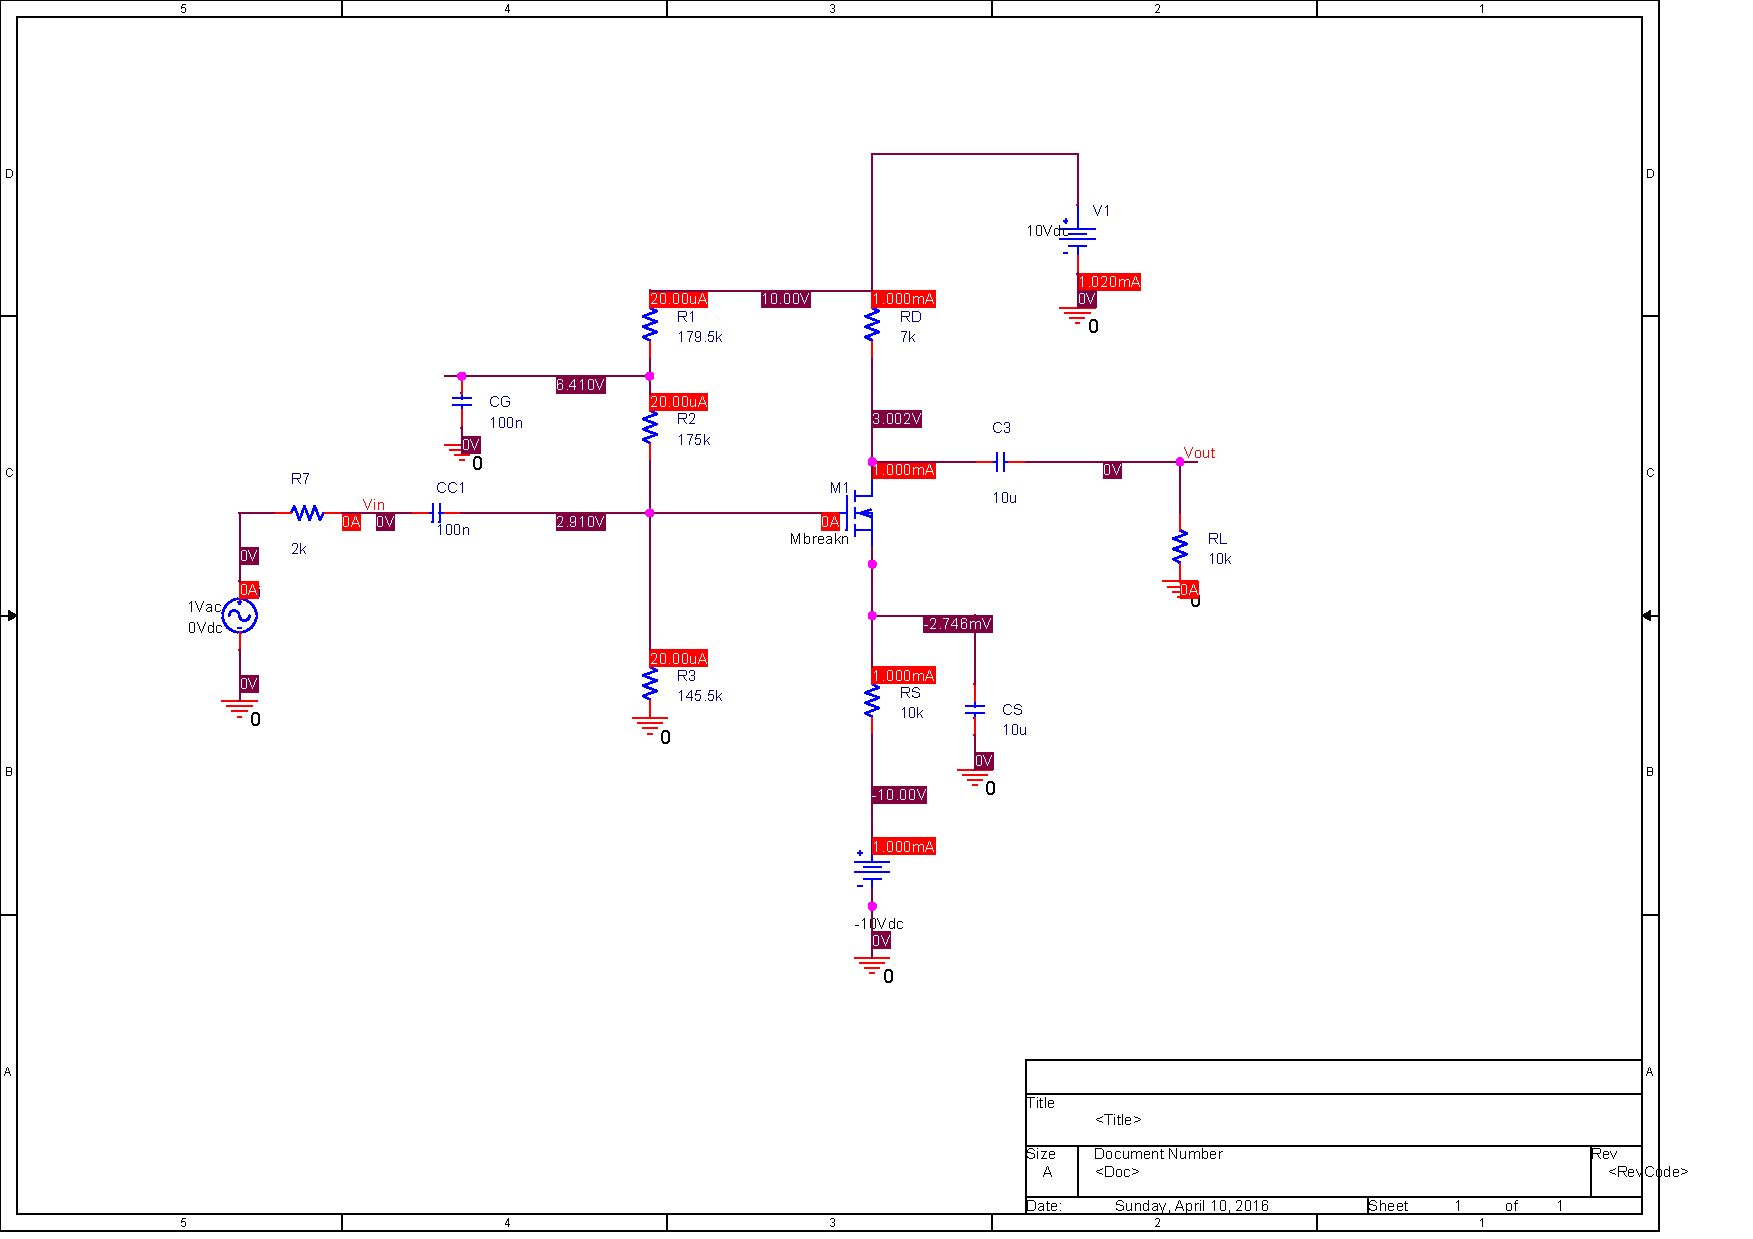
\includegraphics[width=1.00\textwidth]{pic1.pdf}
	\captionof{figure}{Common source amplifier circuit in OrCAD}
\end{figure}

%----------------------------------------------------------------------------------------
%	SECTION 3
%----------------------------------------------------------------------------------------

\section{Discussion}

The hand calculations performed can be seen in the attached document. The gain in the hand calculations came to approximately 9 $\sfrac{V}{V}$, but the output was inverted. Figure 2 shows the results of the frequency sweep. The gain of the simulated circuit is approximately 9 $\sfrac{V}{V}$, however, the output is not inverted (this may simply be an artefact of the software's plotting capabilities).\\

The DC bias values for which the amplifier's bias currents are derived are shown on the OrCAD schematics in Figure 1. These match the hand calculated results almost identically indicating that the simulation provides accurate results. In fact, error in the simulation is not discernible, however, further understanding of divergence between the hand calculated model and simulated model would require a working knowledge of the computational simulation methods employed by OrCAD. It must also be noted that the hand calculation relies on simplification of the non-linear transistor model and hence contains error of its own.


\begin{figure}[H]
	\centering
	\begin{tikzpicture}[scale=1]
	\begin{axis}[
	xmode=log,
	xmin=10, xmax=1000000000,
	ymin=0, ymax=10,
	scale only axis,
	xlabel=Frequency (Hz),
	ylabel={Voltage Gain [$\sfrac{V}{V}$]}
	]
	\addplot [no markers] table [x=X, y=Y, col sep=comma]{./data/data.csv};
	\end{axis}
	\end{tikzpicture}
	\captionof{figure}{Frequency of input voltage versus voltage gain (Note: this plot was made from a pgfplots using a .csv datafile exported from OrCAD)}
\end{figure}

%----------------------------------------------------------------------------------------
%	SECTION 3
%----------------------------------------------------------------------------------------

\section{Conclusion}

The simple common source amplifier was analysed using both hand analysis and a computational approach using software. The DC bias values match perfectly. Further, the magnitude of the gain in the hand calculations matches the simulation. The principal point of difference is that the software did not report an inverted small signal upon amplification.


\end{document}